\documentclass[Japanese,noauthor]{dicomopapers}
\usepackage[dvips]{graphicx}
\usepackage{latexsym}

\def\Underline{\setbox0\hbox\bgroup\let\\\endUnderline}
\def\endUnderline{\vphantom{y}\egroup\smash{\underline{\box0}}\\}
\def\|{\verb|}

%概要投稿用余白調整ここから
\setlength{\Jauthorjreceivesep}{0.0mm}
\setlength{\Jreceivejabstsep}{0.0mm}
\setlength{\Jabstsepjkeyword}{0.0mm}
\setlength{\Jkeywordetitle}{0.0mm}
%概要投稿用余白調整ここまで

\begin{document}

% 和文表題
\title{{\LaTeX}によるDICOMO概要テンプレート}

% 英文表題
\etitle{How to Typeset Your Abstract in {\LaTeX}}

% 所属ラベルの定義
\affiliate{RU}{立命館大学 情報理工学研究科}
\affiliate{JST}{JSTさきがけ}

\author{藤井 敦寛}{ATSUHIRO FUJII}{RU}
\author{村尾 和哉}{KAZUYA MURAO}{RU, JST}

% 表題などの出力
\maketitle

% 本文はここから始まる
\section{研究の背景と目的}
ヘルメットは社会生活において,広く利用されている.中でも,工事現場では大勢が同時に

中尾ら\cite{disaster}の提案する,送受信器,アンテナ及びヘッドホンマイクを取り付けた防災用ヘルメットをはじめ,ウェアラブルデバイス化が



現在スマートカーが注目され,四輪車におけるキーレス化の開発が進む中で,二輪車でのキーレス化は普及していない.そこで二輪車におけるキーレス化に向け,ヘルメットを用いた個人識別手法を提案する.日本国内の公道走行ではヘルメットの着用が義務付けられており,乗車する上で必要な物であるため,これを鍵の代わりに用いる.認証に用いる要素には個人により特徴があり,また偽装が難しいことが重要である.白川らは虹彩と目の周辺画像を統合し認証する手法を提案している\cite{iris_eye}.しかし,目とその周辺画像の取得には目前にカメラが必要であり,ヘルメットに応用するのは難しいため,本研究では個人識別に頭部形状を用いる.ヘルメットを被った際に頭部形状が取得できれば,その差異から個人を識別することが可能であると予想できる.また頭部形状は複製が難しく,認証に適していると考えた.

\section{提案手法}
ヘルメットを被った状態で2[ms]静止し,その間のセンサ値をデータとして蓄積していく.このデータは32個の電圧値を要素とするベクトルであるが,識別に必要なデータは1回被った時に1ベクトルのみであるため,この2[ms]のデータの平均値を用いることとする.また外れ値の影響を考慮し,この32次元ベクトルは主成分分析を行い,2次元に削減する.識別ではデータセットの中で学習データに用いる個数を設定し,学習データの重心を計算する.鍵としての識別ではヘルメットの持ち主であるか,そうでないかを判別するのみであるため,単純に重心から認証データに対する距離により,閾値を用いて判別する.

\section{実装}
実装したプロトタイプデバイスを図\ref{device}に示す.図\ref{device}の左図はプロトタイプデバイスの全体図である.センサ値を正しく取得するには,センサとヘルメット装着者の頭部が密着している必要がある.そのため,フルフェイス型のB\&B社製BB100フルフェイスヘルメットを用いた.ヘルメット内部にはインターリンク エレクトロニクス社製の圧力センサであるFSR402,FSR402 ShortTailを取り付けた.圧力センサは全て並列接続であり,ヘルメット外部に取り付けた10KΩの抵抗を配線してあるプリント基板を経由して,マイコンであるArduino MEGA2560 R3のアナログ入力ポートに接続した.
図\ref{device}の右図はヘルメット内部の様子である.今回用いたヘルメットがフリーサイズで少し大きめであり,内装の脱着が不可能であった.そのため,頭頂部の内装を取り外して,新たに厚みのあるウレタンスポンジを取り付けた.取り付けたウレタンスポンジの中央部に切り込みを入れ,切り込み部分に圧力センサを挿し込んだ.圧力センサは頭頂部に4個,頭頂部周囲に16個,後頭部に6個,左右チークパッド部に6個の合計32個を搭載した.

\section{評価}
提案手法の実現可能性を確認するために,被験者5名(A$\sim$E,全員男性,平均年齢22歳)にプロトタイプデバイスを着用させ,サンプリングレート約30[Hz]で2[ms]間のセンサデータを収集した.2回の着用を1セットとして合計10セットを収集した.1日あたり最大4セットの上限を設定し,データ収集は複数日に渡って実施した.着用によるデバイス位置の差を考慮するため,セット間に休憩時間を設定した.\par
収集したデータを用いて,2次元のデータ量で主成分分析し平面上に描画した結果を図\ref{pca}に示す.図\ref{pca}より,各被験者のデータ群間に明確な散らばりが存在することがわかった.また,装着位置の変化により,各被験者のデータ群内の分散の大きさに差があることがわかった.したがって,各点の距離から装着者を識別することは可能であると考えられる.\par
本評価では,外れ値を考慮するために用いたベクトルのデータ量を32次元から2次元まで削減した.そのため,情報量が大幅に欠落している.したがって,個人の識別に必要な情報まで欠落している可能性がある.提案手法のデータ量の削減方法を検討し直す必要がある.また,図\ref{pca}より,分散が大きいデータ群があったことがわかっている.本実験用に収集したデータが少ないため,追加のデータを収集して評価を行う必要がある.

\section{まとめ}
本研究では,圧力センサを内部に取り付けたヘルメットを着用することで頭部の形状を計測し,頭部の形状差から個人を識別する手法を提案した.評価実験の結果より,個人によりデータ群に差があることが確認できた.今後は,被験者を増やしてデータを収集し,実環境で提案手法の評価をする.また,提案手法の利用者のデータ群に差がないときの個人識別方法を定義する.

\begin{figure}[!t]
  \begin{center}
    \includegraphics[width=1\linewidth]{met.eps}
  \end{center}
  \caption{実装したプロトタイプデバイス}
  \label{device}
\end{figure}

\begin{figure}[!t]
  \begin{center}
    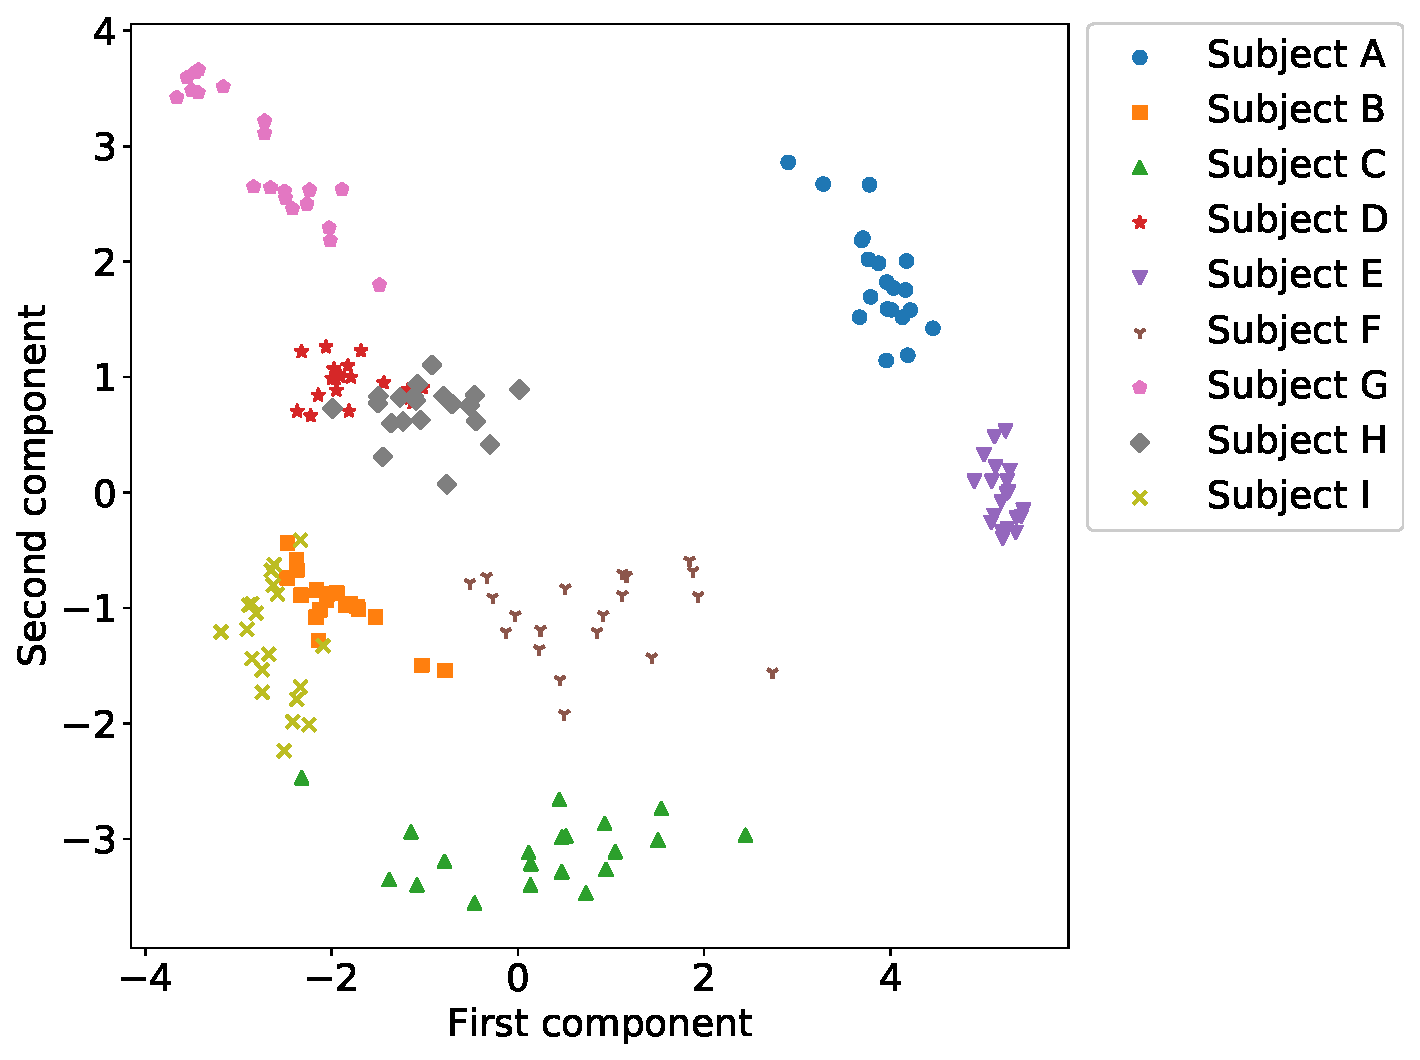
\includegraphics[width=1\linewidth]{PCA.eps}
  \end{center}
  \caption{PCAによる分析結果}
  \label{pca}
\end{figure}

\bibliographystyle{junsrt}
\bibliography{references}

\end{document}
